%!TEX TS-program = pdflatex
%!TeX encoding = UTF-8
%!TeX spellcheck = en_US
%!TeX root = userManual.tex
%!TeX author = Dr.Ing. Mohammed Nour Abdelgwad Ahmed
%!TeX version = 1.5
%!TeX date = 2017.03.10

\documentclass[%
DIV=12,
abstract=on
%a5paper,                 % alle weiteren Papierformat einstellbar
%landscape,              % Querformat
%10pt,                       % Schriftgröße (12pt, 11pt (Standard))
%BCOR1cm,               % Bindekorrektur, bspw. 1 cm
%DIVcalc,                  % führt die Satzspiegelberechnung neu aus scrguide s.2.4
%twoside,                 % Doppelseiten
%twocolumn,            % zweispaltiger Satz
%halfparskip*,           % Absatzformatierung s. scrguide 3.1
%headsepline,           % Trennline zum Seitenkopf
%footsepline,            % Trennline zum Seitenfuß
%titlepage,                % Titelei auf eigener Seite
%normalheadings ,    % Überschriften etwas kleiner (smallheadings)
%idxtotoc,                 % Index im Inhaltsverzeichnis
%liststotoc,               % Abb.- und Tab.verzeichnis im Inhalt
%bibtotoc,                 % Literaturverzeichnis im Inhalt
%abstracton,              % Überschrift über der Zusammenfassung an
%leqno,                      % Nummerierung von Gleichungen links
%fleqn,                       % Ausgabe von Gleichungen linksbündig
%draft                        % überlangen Zeilen in Ausgabe gekennzeichnet
]
{scrartcl} %scrreprt

% Deutsche Anpassungen %
%\usepackage[ngerman]{babel}
\usepackage[T1]{fontenc}
\usepackage[utf8]{inputenc}
\usepackage{lmodern} 	%Type1-Schriftart für nicht-englische Texte
\usepackage{amssymb} %provides various useful mathematical symbols
\usepackage{amsthm}  %provides extended theorem environments
\usepackage{amsmath} %provides the align environment
\usepackage{xcolor}
\usepackage[bookmarks,
  bookmarksopen=false,
  bookmarksnumbered=true,
  pdftex,pdfhighlight=/N,
  linkcolor=blue!60!black,
  urlcolor=blue!60!black,
  colorlinks=true,
  citecolor=green!20!black,
  pdftitle={Steering Control for Autonomous Path Tracking},
  pdfsubject={EO2 Path Following Documentation},  % insert subtitle
  pdfkeywords={terramechanics, testbed, force measurement, soil contact interactions, impedance control, legged robots, simulation},
  pdfauthor={Dr.Ing. Mohammed Nour Abdelgwad Ahmed}]{hyperref}

% Packages für Grafiken & Abbildungen %
\usepackage{graphicx} 	%Zum Laden von Grafiken
%\usepackage{subfig} 	%Teilabbildungen in einer Abbildung
\usepackage{wrapfig}

% Bibliographiestil %
%\usepackage{natbib}

%------------------------------------------------------------------------------
\usepackage[automark,headsepline]{scrlayer-scrpage}
\clearpairofpagestyles
\cfoot[\pagemark]{\pagemark}
\lehead{\headmark}
\rohead{\headmark}
\pagestyle{scrheadings}

%\setkomafont{pagehead}{\normalfont\bfseries}
%\renewcommand*\pagemark{{\usekomafont{pagenumber}Page\nobreakspace\thepage}}
%\addtokomafont{pageheadfoot}{\upshape}
%------------------------------------------------------------------------------


  \usepackage{tikz} %for the revision No. block on the margin of title (first) page
%\usetikzlibrary{shapes}

\definecolor{thegrey} {gray}{0.5}
\definecolor{theshade}{gray}{0.94}
\definecolor{theframe}{gray}{0.75}

\usepackage{myboxedtheorem}
%\newboxedtheorem[options]{theo}{Theorem}{thCounter}
%boxcolor = black, titleboxcolor = black, background = white, titlebackground = white, titlecolor = black, thcounter=, size = .9\textwidth
%\newboxedtheorem[boxcolor=blue!20, background=blue!5, titlebackground=blue!20, titleboxcolor = blue!20]{theo}{Theorem}{anything}
\newboxedtheorem[boxcolor=theframe, background=theshade, titlebackground=thegrey,%
                 titlecolor = white, titleboxcolor = thegrey, size = 0.8\textwidth]{myColoredBox}{}{}

\newboxedtheorem[boxcolor=pink, titleboxcolor = pink, titlebackground=red!20, background=red!5]{mytheo}{}{}
%------------------------------------------------------------------------------
\setkomafont{title}{\normalfont\bfseries\small} %to set the tile font (I hate the default one ;))

\graphicspath{{./figures/}}
\pagestyle{empty} %Keine Kopf-/Fusszeilen auf den ersten Seiten.
%==============================================================================
%==============================================================================

\begin{document}
\thispagestyle{scrplain}

% title page ------------------------------------------------------------------
\titlehead{Titelkopf}
\subject{EO2 Path Following Documentation}
\title{EO2 Intelligent Driving Assistance (IDA)}
\subtitle{Steering Control for Autonomous Path Tracking}
\author{Dr.Ing. Mohammed Nour\footnote{corresponding author: Zagazig University, Faculty of Engineering, Computer and Systems Dept., Zagazig, Egypt, \href{mailto:mnahmed@eng.zu.edu.eg}{mnahmed@eng.zu.edu.eg}} %{Mohammed Ahmed}
\and{Eng. Zaid Obeid}
\and{Eng. Folan Ellan}
\and{Eng. Zaid Obeid2}
\and{Eng. Folan Ellan2}
\and{Eng. Folan Ellan3}
}
%\thanks{last revision \today}           % entspr. \footnote im Fließtext
\date{}%\today}                                 % in case another date other than today is wanted

\publishers{\vspace{15 mm}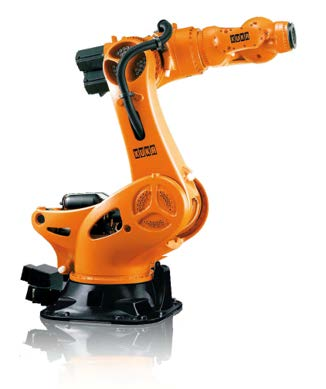
\includegraphics[width=0.55\textwidth]{kuka}}

% dedication ------------------------------------------------------------------
%\dedication{Widmung}

\maketitle      % show the title page

% add the revison side block
\begin{tikzpicture}[overlay,remember picture]
  \node[fill=black!30,text=white, inner ysep=2pt, inner xsep=20pt, rectangle,rotate=90]
    at ([xshift=10mm,yshift=0mm]current page.west)
    {\footnotesize{last revision \today}};
\end{tikzpicture}
%==============================================================================
% abstract after title and befor table of contents 
\vfill
\begin{abstract}
This report presents the derivation, design, and implementation of the ZUKA project.
\end{abstract}

%==============================================================================
\clearpage
\pagestyle{scrheadings}
\tableofcontents
%\listoftables
%\listoffigures
%\newpage
\clearpage
%==============================================================================

% main content ----------------------------------------------------------------
\section{Path Following Module }
where $(x, y)$ represents the coordinates of the point $P$ located at mid-distance of the actuated wheels, the angle $\theta$ characterizes the vehicle chassis orientation, $\phi$ represents the vehicle steering \textbf{wheel} angle, and $L$ is the distance between the rear and front wheels axles.
%------------------------------------------------------------------------------

\subsection{Vehicle Model}
For the vehicle, the kinematic model used (shown in Fig.\ref{fig:configurationVariables}) is:
\begin{align}
\dot{x} &= u_1 \cos\theta \notag\\
\dot{y} &= u_1 \sin\theta \notag\\
\dot{\theta} &=\frac{u_1 }{L} \tan\phi \notag\\
\dot{\phi} &= u_2
\label{eq:kinematicModel}
\end{align}
where $(x, y)$ represents the coordinates of the point $P$ located at mid-distance of the actuated wheels, the angle $\theta$ characterizes the vehicle chassis orientation, $\phi$ represents the vehicle steering wheel angle, and $L$ is the distance between the rear and front wheels axles.
\begin{figure}[htbp]
	\centering
    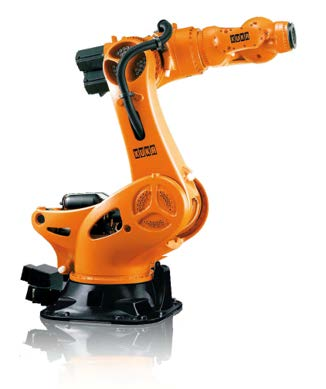
\includegraphics[width=0.4\textwidth]{kuka}
    \caption{Configuration variables of the vehicle kinematic model}
	\label{fig:configurationVariables}
\end{figure}

 \begin{mytheo}[$\looparrowright$ Law of Large Numbers]
    To calculate the horizontal position the kinematic differential equations are needed:
    \begin{align}
    \dot{n} &= u\cos\psi -v\sin\psi \\
    \dot{e} &= u\sin\psi + v\cos\psi
    \end{align}
\end{mytheo}
%==============================================================================

\newpage
\appendix
\section{Appendix Part }
where $(x, y)$ represents the coordinates of the point $P$ located at mid-distance of the actuated wheels, the angle $\theta$ characterizes the vehicle chassis orientation, $\phi$ represents the vehicle steering wheel angle, and $L$ is the distance between the rear and front wheels axles.
\end{document}
